\documentclass[12pt,a4	]{report}
\usepackage[frenchb]{babel}
\usepackage[usenames,dvipsnames]{color}
\usepackage[utf8]{inputenc}
\usepackage{textcomp}
\usepackage[T1]{fontenc}
\usepackage{lmodern}	
\usepackage{bibunits}
\usepackage{graphicx}
\usepackage{wrapfig}
\usepackage{glossaries}
\usepackage{float}
\usepackage{cite}
\usepackage{caption}
\usepackage{amsmath,mathtools}
\usepackage{subcaption}

\begin{document}
\chapter{Contribution}
\section{Ouverture}
\paragraph{}
Les articles de Wikipédia sont constitués généralement d'un texte, mais aussi de certaines informations structurées (infobox, images, liens externes, redirections entre les pages etc...) présentes sous la forme de balises Wiki. 
Le projet DBpedia extrait des informations structurées de Wikipédia et les transforme dans une base de connaissances riche sous forme d'un graphe avec des entités reliées.
\subparagraph{}
Dans ce chapitre, nous allons vous donné une vue d'ensemble sur l'annotation des métadonnées, une analyse des besoins, la procédure d'extraction de DBpedia et les pistes de travail possibles. Puis nous présenterons l'architecture globale de notre système ainsi que notre hypothèse et la structure de l'application que nous avons développée pour concrétiser notre hypothèse. La dernière partie de cette section porte sur les résulats de cette étude.
\section{Utilité des annotations}
\paragraph{}
En générale, l'annotation, c'est une étiquette qu'on ajoute à une ressource Web. Depuis la création du Web, plusieurs systèmes d'annotation sont apparus (ThirdVoice, PageSeeder, HyperNews, Nestor, etc...).
Nous citons brièvement les conséquences liées à ces systèmes d'annotation telles que l'information annotée doit d'une manière ou d'une autre être structurée, utilisable et descriptive de la ressource ou de son utilisation. De plus, la ressource en question doit exister et peut être exploitée sur le Web indépendamment des informations qui lui sont associées. La figure ci-dessous montre le système intermédiaire entre le client et le service Web dans lequel il y a le service de gestion des annotations, permettant la communication entre ces deux entités.
\begin{figure}[H]
\centering
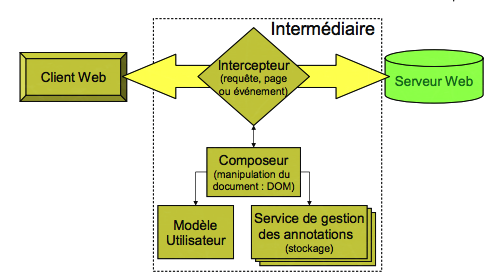
\includegraphics[width=11cm]{AnnotationSys.png}
\caption{Notation d'intermédiaire}
\end{figure}
\subparagraph{}
L'annotation sémantique faite référence à plusieurs types distincts d'annotations formelles, explicites et permanentes. Il existe des outils d'annotation basés sur les ontologies {\it Ontology based annotation tool}
et des critères relatifs aux annotations par exemple : les types de ressources concernées, la structuration des schémas de description, l'automatisation marquée de la mise en place, etc.
\begin{figure}[H]
\centering
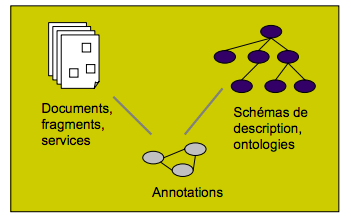
\includegraphics[width=9cm]{diffConnaissances.png}
\caption{Différents niveaux de connaissances}
\end{figure}
\subparagraph{}
L'annotation d'un triplet RDF est une façon d'ajouter des metadonnées à un triplet RDF pour décrire une restriction spatiale.
\newline
\textit{Comment on utilise les annotations temporelles ?} Un exemple d'utilisation est sur le site ``sig.ma''\footnote{http://sig.ma/} crée par \textit{the digital enterprise research institute in Ireland}, la plateforme fournit un moteur de recherche par mot clé qui permet de récupérer des images et des textes accessibles par des annotations RDF, ainsi qu'une liste d'URI synonymes correspondant à la clé de recherche et des liens vers des sources Web contenant des données RDF pertinentes.
\section{Analyse des Besoins}
\paragraph{}
Le large succès de Wikipedia (qui est le 2éme site le plus visité sur internet) et le progrès des techniques d’extraction des données ont abouti à la naissance de la construction automatique  de larges bases de connaissances comme DBpedia, YAGO, etc...
\begin{figure}[H]
\centering
\includegraphics[width=10cm]{Sources.png}
\caption{Différentes sources d'informations dans DBpedia}
\end{figure}
\subparagraph{}
Beaucoup de connaissances sont construites en se basant sur l’extraction automatique des faits relationnels dans un texte.
En effet, les bases de connaissances convergent sur les faits statiques et ne donnent pas une grande importance à la dimension temporelle de ces triplets.
Et ceci a lieu en dépit du fait que la majorité des faits évoluent avec le temps, ou ne sont valides que dans une période temporelle précise. Ainsi, nous remarquons que le temps a une dimension significative dans ces bases de connaissances.
\subparagraph{}
La dimension temporelle est particulièrement importante dans les relations binaires comme $isPresidentOf$, $isCEOof$, $isMarriedTo$, on peut être mariée à plusieurs épouses mais dans des différents intervalles de temps (On ne tiens pas compte des exceptions que représentent les mariages polygames).
Une base de connaissances contenant plusieurs présidents des États-Unis ne peut être consistante que lorsqu’on ajoute une dimension temporelle à ces faits. De plus l’annotation temporelle aide à faire la distinction entre les faits courants et les faits dépassés.
Par exemple le fait ``Kennedy est le président des États-Unis'' est correct, mais n'est plus valide.
Lorsqu’on attache une annotation temporelle à un fait comme celui là, il devient universellement valide.

\section{Problèmatique}
\paragraph{}
Lorsqu’on parcourt DBpedia, on trouve beaucoup de triplets qui décrivent des informations temporelles. Ces derniers sont généralement liés à un contexte événementiel précis.
Il est plus difficile d’exploiter ces informations si elles ne possèdent pas une structure universellement valide, claire et lisible par la machine. Dans DBpedia, il se trouve que des informations liées au même contexte temporel sont exprimées de la manière suivante : 
\begin{figure}[H]
        \centering
                \centering
                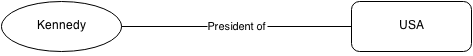
\includegraphics[width=10cm]{ken.png}
               \caption{triplet ''Kennedy''}

\end{figure}
\subparagraph{}
Le premier triplet n'a pas une sémantique valide que en tenant compte du triplet suivant~: 
\begin{figure}[H]
        \centering
                \centering
                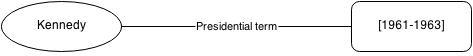
\includegraphics[width=10cm]{presidterm.png}
               \caption{triplet presidential term ''Kennedy''}

\end{figure}
\subparagraph{}
Dans cette étude, on vise plutôt à annoter les triplets ($s$, $p$, $o$) avec une étiquette temporelle qui indique et précise la validité de ce terme dans un cadre logique qui appartient au monde réel où en dehors de ce cadre, on peut dire que ce triplet RDF n’est pas valide et qu’on ne peut pas l’utiliser.

\section{Étude préliminaire et approches possibles}
\subsection{Web Collaboratif}
\paragraph{}
C'est le Web qui s'appuie sur les utilisateurs pour construire son contenu. Nous avons commencé notre travail de recherche par une étude préliminaire autour du contenu de ces plateformes collaboratives. Aussi, nous avons étudié les pistes possibles pour l'exploitation des dumps de Wikipédia et Wikidata. Tout d'abord, nous avons téléchargé les fichiers des collections XML et nous avons observé la structure des informations dans ces sources d'informations. Ensuite nous avons implémenté un premier algorithme d'extraction en utilisant un parseur XML (SAX\footnote{http://fr.wikipedia.org/wiki/Simple\_API\_for\_XML}).
La figure ci-dessous représente notre schéma de modélisation dans lequel nous avons procédé avec une modélisation qui touche directement la source principale d'informations Wikipédia.
\begin{figure}[H]
        \centering
                \centering
                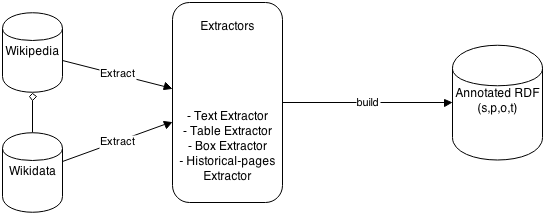
\includegraphics[width=10cm]{modelisation.png}
               \caption{Première approche : schéma de modélisation générale}

\end{figure}
\subparagraph{}
Cette modélisation est une première rubrique d'analyse et de conception d'une solution qui touche les besoins préliminaires de notre étude. Par ailleurs, nous avons retrouvé une autre modélisation plus proche à nos besoins principaux et que nous vous détaillerons par la suite.
\subsection{Traitement automatique des langues}
\paragraph{}
Le traitement automatique de la langue (TAL) est une discipline à la frontière de la linguistique, qui est intimement liée à l'intelligence artificielle.
Il existait un type de TAL statistique proposent des méthodes statistiques, probabilistes ou purement statistiques pour résoudre pour résoudre certaines difficultés.
On distingue plusieurs domaines d'application de TAL comme la traduction automatique, la génération automatique de texte, la correction orthographique, la reconnaissance de l'écriture manuscrite, etc...
Mais dans ce type de traitement, il y a des problèmes qui peuvent apparaître et principalement celui de l'ambiguïté temporelle.

\subsection{Ambiguïtés temporelles}
\paragraph{}
C'est la propriété d'un mot ou d'une suite de mots (comme notre cas) qui peuvent avoir un ou plusieurs sens d'analyses grammaticales possibles. Dans une phrase simple ou composée, l'indicateur temporel peut avoir plusieurs sens tout dépend du contexte de la phrase.
\newline
Les informations temporelles peuvent avoir des représentations différentes~: 
\begin{itemize}
\item Un évènement ``Je vous propose un rendez-vous $demain$ pour parler de ma plateforme PiSharing''. \item Une connaissance ``Jacques Chirac est le président de la république Française'' \textbf{ mais quand ?}.
\end{itemize}

\subparagraph{} 
Le présent par exemple peut avoir plusieurs sens ou contextes : présent de narration, présent de généralité, présent qui réfère au futur proche, etc...
Les signaux temporels sont ambigus par exemple dans ces expressions : il court pour rattraper le temps, tu tournes après la rivière, etc… On remarque qu'il y a des indicateurs temporels, mais ce n'est pas le temps qui est relatif à un événement qui peut nous intéresser.
La plupart des expressions sont floues comme: il y a deux ans, chaque deux semaines, j’arrive dans deux secondes, etc... En effet, il n'y a pas une logique descriptive qui peut nous aider à mettre un le lien entre l'événement et la période temporelle.
\paragraph{}
L’analyse du temps s’inscrit dans la compréhension globale des textes, et des évènements auxquels on fait référence dans ce texte non pas en analysant une phrase comme suit. 
\newline
Modalité~: ``l’équipe de France voulait gagner la coupe du monde en 2006.'' 
\newline
Anaphore~:  ``..., cela pourrait avoir lieu dans les éditions suivantes.''
\subparagraph{}
Les évènements décrits (et que l’on souhaite fixer temporellement) peuvent être : duratifs ou ponctuels/accomplis ou inaccomplis. 
De même pour les dates qui peuvent être des dates absolues ``le 18 mars, c'est mon anniversaire'' ; ou bien des dates relatives par rapport au moment de l’énonciation par exemple : ``il y a deux ans''. Pour la durée aussi on distingue plusieurs types comme la durée absolue ``durant 2 ans'' et la durée relative ``depuis un an''. Dans un texte, on trouve aussi un ensemble d'expressions de fréquence comme ``tous les ans, le vendredi 13'' et des expressions plus complexes comme ``après la Révolution Tunisienne''.
\subparagraph{}
Les textes contiennent des informations temporelles de taille massive qui sont difficilement exploitables. Nous avons donné une vue globale sur cette procédure que nous avons décidé de ne pas l'adopter parce que notre objectif est d'annoter des triplets RDF plutôt que de faire l'analyse des textes. Nous détaillerons par la suite l'architecture de DBpedia à partir de laquelle on s'inspire pour proposer notre solution.
\subsection{Historique des modifications dans Wikipédia}
\paragraph{}
L'historique est une page attachée à un article encyclopédique pour conserver le journal de la plupart des modifications qui ont été apportées à cet article. Cette page permet de connaître la date, l'auteur et la teneur externe de chaque modification.
Dans cette encyclopédie, nous avons remarqué qu'à partir de l'historique de modifications, on peut déduire plusieurs informations liées à deux ou plusieurs contextes temporels différents.
Nous souhaitons, si c’est possible, extraire ces informations temporelles et les rendre exploitables dans DBpedia.
\begin{figure}[H]
\centering
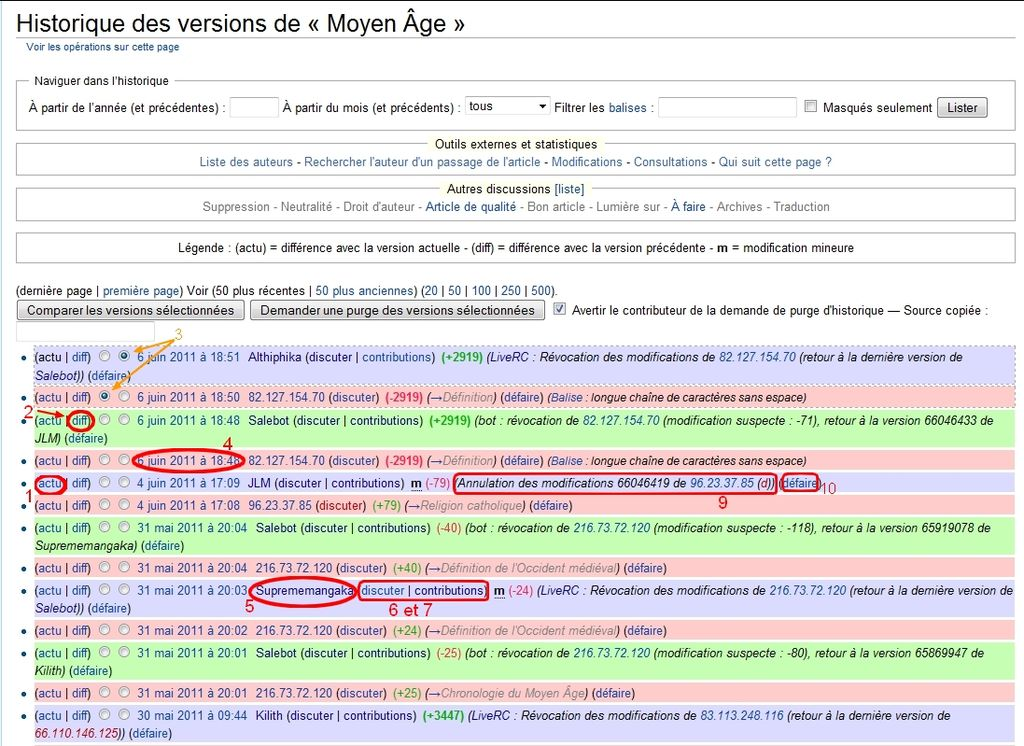
\includegraphics[width=13cm]{Historique_articles.jpg}
\caption{Historique d'articles Wikipédia}
\end{figure}
\newpage

\section{Architecture d'extraction de DBpedia}
\subsection{Vue d'ensemble}
\begin{figure}[H]
\centering
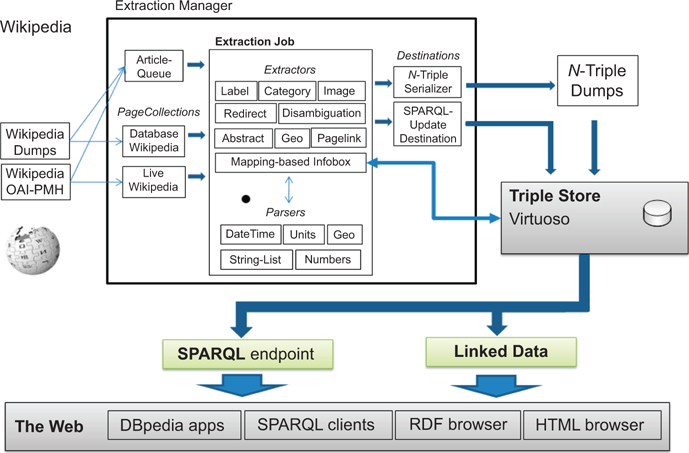
\includegraphics[width=12cm]{dbpediaExtra.png}
\caption{Extracteur DBpedia}
\end{figure}
La figure ci-dessus montre l'architecture du système d'extraction des connaissances dans DBpedia.
D'apres Morsey et al~\cite{morsey2012} les principaux éléments du système sont les suivants : $PageCollections$ est une abstraction des ressources locales ou distantes des articles de Wikipédia, $Collections$ stokent ou sérialisent les triplets RDF extraites, $Extractors$ qui transforme un type spécifique de la syntaxe wiki en triplet, $Parsers$ soutiennent les $Extractors$ en déterminant les types de données, convertit les valeurs entre différentes unités et fractionne les marqueurs dans des listes. L'$Extraction$ $Job$ regroupe une collection de pages, extracteurs et destination dans le flux de travail $workflow$.
Le noyau de ce système est l'$Extraction$ $Manager$ qui gère le processus  d'adoption des articles de Wikipédia sur les $Extractors$ et donne les résultats à la destination.
Le gestionnaire d'extraction $Extraction$ $Manager$ gère également la gestion des URI et résout les redirections entre les articles : ce système se compose de $11$ extracteurs qui traitent les types des contenus de Wikipédia ($Labels$, $Abstracts$, $Interlanguage$ $links$, $Images$, $Redirects$, $Disambiguation$,
$External$ $Links$, $Pagelinks$, $Homepages$, $Categories$, $Geo-coordinates$).
Ce framework d'extraction DBpedia est mise en place pour réaliser deux flux : extraction à partir des sources de données ($DataBaseWikipedia$ $page$ $collections$) et une procédure d'extraction directe
($LiveWikipedia$ $page$ $collections$ $with$ $the$ $OAI-PMH$ $protocol$) pour obtenir la version courante des articles.
\subsection{Notre proposition}
\paragraph{}
En analysant les $dumps$ DBpedia et en observant l'architecture de cette base de connaissance, nous avons remarqué que pour annoter temporellement les triplets RDF de DBpedia il est plus intéressant d'extraire l'ensemble des propriétés dans DBpedia, puis de trouver des faits qui ont un trait avec le temps, donner une liste de couples à partir de laquelle un expert choisit un couple et valide les résultats de notre algorithme. Par la suite, nous allons présenter en détail notre proposition.
\subsection{Modélisation}
\paragraph{}
Le modèle quaternaire est un modèle qui capte la base du fait avec un indice temporel, l'exemple suivant en montre le principe de ce modèle.
\newline
{\it <politician> elected <president of US> on <date>}
\newline
f1, Kennedy elected PresidentOfUSA 
\newline
f2:f1, HappenedDate
\newline
{\it <politician> served as <politician office> from <date> to <date>}
\newline
f1, Kennedy holdsPoliticalPosition PresidentOfUSA 
\newline
f2:f1, startedOnDate 
\newline
f3:f1, endedOnDate
\newline
$HappenedDate$ est utilisée pour dire que le fait est valide que dans ce point du temps.
\begin{figure}[H]
        \centering
                \centering
                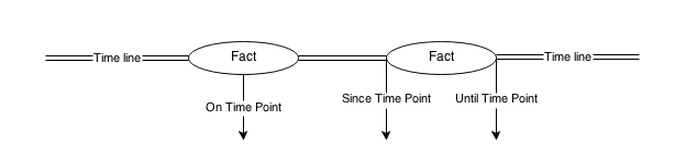
\includegraphics[width=13cm]{timeline.png}
               \caption{Chronologie des événements}

\end{figure}
\subparagraph{}
Ce modèle est capable d'exprimer la validité temporelle d’un triplet RDF d’une manière à la fois intelligente et lisible par la machine ; on souhaite rattacher au triplet valide que dans un point du temps ou une plage temporelle bien précise une étiquette temporelle adéquate comme le montre la figure suivante.
\begin{figure}[H]
        \centering
                \centering
                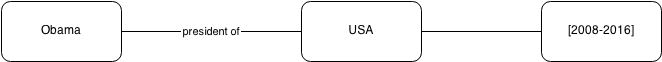
\includegraphics[width=10cm]{obamaQuad.png}
               \caption{Modélisation quadruplet}

\end{figure}
\subparagraph{}
On s'intéresse particulièrement au format N-Quads comme format de sortie de notre algorithme. Les quadruplets vont être formalisés de la manière suivante~:
\newline
$<s,p,o,t>$ : un sujet, prédicat, objet avec un point de temps.
\newline
$<s,p,o,[t1,t2]>$ : de même avec une intervalle de temps.
\subsection{Notre hypothèse}
\paragraph{}
Après une observation approfondie dans les sources de données dans DBpédia, nous avons repéré des relations logiques entre des propriétés comme ($beatifiedBy$, $beatifiedDate$). Nous avons trouvé plusieurs propriétés qui ont un lien logique entre eux, les relations temporelles ont comme objet un point du temps particulier et partagent le même sujet ou la même ressource avec une autre propriété.
Durant cette étude nous avons essayé de valider cette hypothèse :

\begin{verbatim}
if (x propTemp t) and (x propWithToken z) then
             (x propWithToken z) t 
\end{verbatim}

\subparagraph{}

$propTemp$ est une propriété DBpédia contenant un indice temporel (Year, Date).
\newline
$propWithToken$ est une propriété DBpédia avec un motif rattacher.
\newline
$t$ est l'annotation temporelle du triplet ($x$,$propWithToken$,$z$).

\subparagraph{}
Nous avons présenté cette hypothèse sous forme d'une requête SPARQL. Cette requête interroge l'ensemble des ressources sur DBpédia et retourne des résultats si c'est possible.
Notre hypothèse porte principalement sur le fait d'annoté temporellement les ressources de DBpedia en utilisant en essayant de repérer deux triplets portent sur un même sujet et permettant à les relier dont le but est d'avoir un quadruplet valide. La liste des couples ($PropTemp$, $PropWithToken$)
est donnée comme sortie d'une procédure d'extraction intelligente de l'ensemble des propriétés de DBpédia.
\section{Notre choix}
\subsection{Architecture du système}
 \begin{figure}[H]
        \centering
                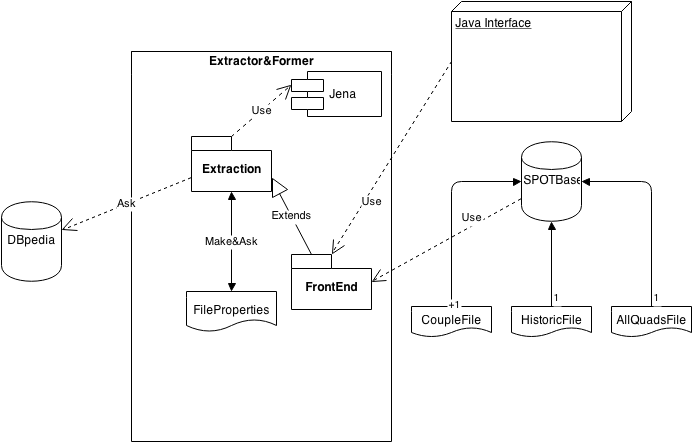
\includegraphics[width=11cm]{Architecture.png}
               \caption{Architecture de l'application}
\end{figure}
\paragraph{}
L'architecture de notre application se repose principalement sur celle de DBpédia. En premier lieu, nous interrogeons DBpédia pour avoir une liste de propriétés. En effet, nous pouvons prendre la liste de toutes les propriétés en interrogant $Virtuoso$ $SPARQL$ $Query$ $Editor$\footnote{http://dbpedia.org/sparql}  avec la requête \begin{verbatim} select distinct ?P where {?S ?P ?O},\end{verbatim}mais on se limite aux propriétés de DBpedia qui ont la forme suivante \begin{verbatim} ?S rdfs:domain ?O \end{verbatim} $rdfs:domain$ est une instance de $rdfs:Property$ qui est utilisé pour indiquer que toute ressource qui possède une propriété donnée est une instance d'une ou plusieurs classes. Le triplet précédant indique que, $S$ est une instance de la classe $rdf:Property$, $O$ est une instance de la classe $rdfs:Class$ et les ressources désignées par les sujets des triplets dont le prédicat est $S$ sont des instances de la classe $O$. Lorsque une propriété $S$ a plus d'une propriété $rdfs:domain$, les ressources indiquées par les sujets des triplets avec prédicat $S$ sont des instances de toutes les classes indiquées par les propriétés $rdfs:domain$. $rdfs:domain$ peut être appliqués à lui-même. $rdfs:domain$ de $rdfs:domain$ est la classe $rdfs:Property$. Cela veut dire que toute ressource avec une propriété $rdfs:domain$ est une instance de $rdf:Property$. 
\subparagraph{}
Ensuite, nous avons choisi de stocker l'ensemble de propriétés dans un fichier pour ne pas avoir des contraintes de mémoire (stockage dans la mémoire vive) et pour ne pas interroger la base de connaissance à chaque fois. Cette procédure se fait une seule fois l'hors du premier lancement de l'application et elle ne sera plus nécessaire après, car il suffit de spécifier le nom du fichier des propriétés DBpédia que nous avons utilisé l'hors de la première exécution, mais nous avons mis la possibilité d'extraction et mise à jour de ce fichier parce qu'il se trouve que DBpédia change quotidiennement et il y a des propriétés qui s'ajoutent au fur et à mesure à cette base de connaissance. Puis, à partir de ces propriétés, nous avons implémenté un algorithme d'extraction qui à comme sortie une liste de couples de propriétés (PropriétéTemporelle, PropriétéReliée). Dans l'application, nous avons choisi de prendre l'avis d'un expert pour valider les résultats de notre algorithme à travers une liste labellisée d'une partie des quadruplets que nous avons réussi à former et à extraire automatiquement dans un $output$ $Textarea$. Nous avons écrit notre hypothèse de base sous forme d'une requête SPARQL de la manière suivante :
\begin{verbatim}
PREFIX rdfs: <http://www.w3.org/2000/01/rdf-schema#> 
PREFIX dbp:<http://dbpedia.org/ontology/> 
SELECT CONCAT(?label1, relatedProp , ?label2, ' : ', ?date) 
			WHERE {  
					 ?S   		dbp:relatedProp 	 ?O;
							dbp:tempProp		 ?date;
							rdfs:label 			 ?label1.
					?O 		rdfs:label ?label2.
					FILTER(lang(?label1)='en' && lang(?label2)='en'}
\end{verbatim}
{\it - tempProp est une propriété temporelle proposé.}
\newline
{\it - relatedProp est une propriété reliée à tempProp partage avec elle un même motif ``Token''.}
\subparagraph{}
L'objectif de cette procédure est de permettre à l'expert de valider ou ne pas valider la logique de la représentation des quadruplets. Enfin, la validation des résultats permet de stocker l'ensemble des résultats (triplets annotés) dans un fichier portant les labels du couple et un autre fichier ``allQuadsFile'' contenant tous les quadruplets validés. Par la suite, notre algorithme fait automatiquement l'appel à un fichier CSV d'historique qui a forme suivante 
\newline
{\tt (attribute,tempAttribute,boolean,date\_Exploration,keep,file)} 
\newline
Où $attribute$ et $tempAttribute$ représentent le couple de propriétés DBpédia, $boolean$ peut être $0$ ou $1$ qui désignent respectivement la volonté de l'expert de valider ou ne pas validé les résultats, $date\_Exploration$ est la date de l'exploration. $keep$ représente le nombre de quadruplets que nous avons formé à partir du triplet et $file$ est le nom de fichier dans lequel nous avons stocké les résultats.
Ce fichier nous permet d'avoir une vision globale sur les résultats de notre étude.
L'ensemble de fichiers seront stockés dans un dossier forment une base de données de sortie que nous avons appelé SPOTBase.
\subsection{Analyse et discussion}
\paragraph{}
Nous avons réussi à former $305$ couples de propriétés, mais nous pouvons encore restreindre ce nombre. Dans notre méthode, nous avons choisi d'extraire même les propriétés reliées aux propriétés temporelles qui contiennent un motif similaire et non pas seulement qui sont identique au suffixe d'une propriété temporelle. Cela a été dans la mesure d'augmenter le nombre de nos données de test pour avoir une vision globale sur les propriétés DBpédia et analyser par la suite les différents résultats/possibilités. 
\subparagraph{}
Avec certains couples, nous avons eu des très bons résultats, par exemple avec le couple ($deathCause$,$deathYear$) nous avons réussi à formé $2766$ quads. La figure ci-dessous montre le format de la sortie de notre algorithme.
 \begin{figure}[H]
        \centering
                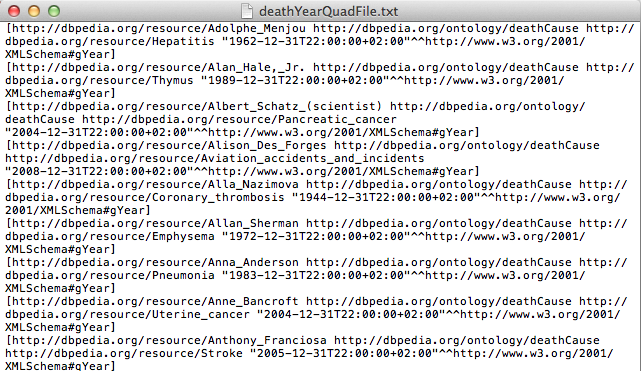
\includegraphics[width=13cm]{DeathYearCause.png}
               \caption{Fichier de Quadruplet DeathYear et DeathCause}
\end{figure}
\subparagraph{}
Il se trouve aussi qu'il y a des couples qui valident notre hypothèse mais qui ne donnent pas de résultats. Il se peut que les deux triplets ne partagent pas le même sujet comme \{(wineRegion, wineYear),(whaDraft, whaDraftYear),(areaCode, areaDate), etc...\}
\newpage
\section{Outils}
\subsection{Application Java}
\paragraph{}
Le choix de développer le logiciel sous forme d'une application $Java$ était un choix personnel et qui s'explique de nombreuses manières. Premièrement, la maîtrise de ce langage de programmation me permet d'utiliser des différentes structures de données et d'explorer la documentation de certaines méthodes plus facilement. De plus, il existe plusieurs sources de documentation sur le Web. En outre une large communauté aide à répondre aux questions si jamais on rencontre des difficultés. Il existe une version Java de DBpédia et cela permet plus facilement d'intégrer mon application open source et disponible sur mon compte\footnote{https://github.com/metanote/Extraction} github. Enfin, nous avons utilisé les librairies $Jena$ qui sont aussi écrites en Java. 
\subsection{Jena}
Jena\footnote{https://jena.apache.org/} est un $Framework$ open source écrit en Java pour construire des applications dans les domaines du
$LinkedData$ et le Web sémantique. Nous avons utilisé les différentes librairies des ce $Framework$ pour interroger DBpédia avec des requêtes SPARQL. $Jena$ est composé de plusieurs programmes différents qui interagissent entre eux pour traiter des données écrites en RDF. $Jena$ fournit un support pour le langage de définition d'ontologies (OWL). Ce $Framework$ se compose des différentes API RDF, Ontology et SPARQL. Une couche interface d'application et une troisième couche pour le stockage. La figure ci-dessous présente en détaille les différentes composantes de Jena.
 \begin{figure}[H]
        \centering
                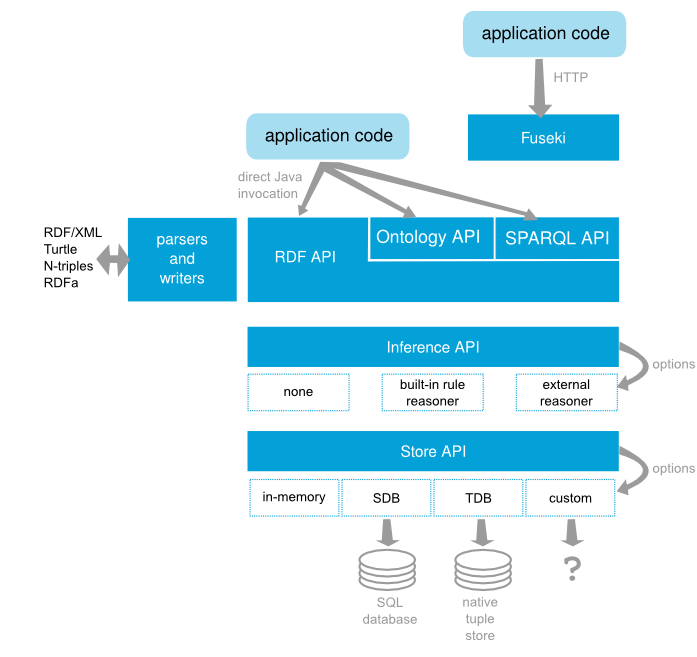
\includegraphics[width=12cm]{Jena.png}
               \caption{Jena Interaction entre les différents API}
\end{figure}
\subsection{Résultats et Validation}
\paragraph{}
Durant cette étude, nous avons essayé d'annoter temporellement des triplets DBpedia. Nous avons réussi à former automatiquement un nombre important de quadruplet à partir de couple de propriétés qui valide notre hypthèse. Pour certaines propriétés, notre programme prend une quinzaine de minutes des fois pour donner des résultats. Sachant qu'on utilise une machine sous OS x avec un processeur $2$ GHz Intel Core i$7$ er $8$ GO de mémoire. Cela est dû au nombre gigantesque de triplets qu'on interroge.
\subparagraph{}
Nous avons stocké plus que $106998$ quads que nous avons réussi à former dans le fichier $AllQaudsFile$. Nous avons remarqué que certains couples valident bien notre hypothèse et donne des excellents résultats. Certes, il y a d'autres couples ne donnent aucun résultat. Le problème, c'est que toutes les propriétés DBpédia ne suivent pas toujours la même logique de représentation. Si tel n'était pas le cas, nous pouvons avoir beaucoup plus de résultats.
Dans le Web sémantique, nous avons remarqué qu'il est très important de mettre des conventions pour la représentation des données. Cela permet non seulement d'utiliser les triplets existants, mais aussi de mettre des hypothèses permettant de construire des travaux au dessus de ce qui existait. Le Web sémantique évolue s'il se repose sur une structure de métadonnées générique, claire et réutilisable. Dans cette étude, nous avons traité des triplets DBpédia. Nous avons réussi à implémenter une solution pour annoter des triplets qui ont un trait avec le temps et nous avons mis ces triplets sous la forme quadruplet. Nous avons manipulé une partie de triplets de la base de données d'entrer pour construire notre base de données quadruplets de sortie que nous avons appelé SPOTBase.
\section{Résumé}
\paragraph{}
Dans cette section, nous avons présenté notre approche à travers un système d'annotation temporelle des triplets dans DBpédia que nous avons développé. Dans un premier lieu, nous avons effectué une étude préliminaire en analysant les besoins et en étudiant l'architecture de la base de connaissance.
Par la suite, nous avons proposé une solution que nous avons implémenté sous forme d'un prototype fonctionnel.
\subparagraph{}
Dans la prochaine section, nous présenterons les perspectives et les pistes d'amélioration possibles. On conclut ce travail avec un récapitulatif qui résume la richesse de cette étude et son apport considérable dans le domaine de l'ingénierie et la recherche.  
\bibliography{Biblio.bib}
\end{document}